% !TEX root = ../report.tex

\chapter{Proposed ADC Architecture}
\label{sec:HadamardADC}

The proposed architecture is based on the Hadamard ADC that was proposed by Malmberg in \cite{malmberg_thesis} and \cite{malmberg_talk}. The main objective of the Hadamard ADC is to distribute the mismatch sensitivity equally among all involved circuit components. In addition, the Hadamard ADC enables a beneficial way of combining multiple input channels. The properties of the Hadamard ADC will be further explored later in this chapter.

The key idea of the Hadamard ADC is to separate the logical states from the physical ones. This is done by applying a Hadamard transform to the input signal vector before the integration. This way, the \textit{physical} states entering each integrator contains an orthogonal mixture of each of the input channels, i.e. the state space is rotated.

A hardware architecture for this Hadamard system is presented in \cite{malmberg_thesis} and \cite{malmberg_talk}. This architecture has good mismatch properties and performs very well in combination with overcomplete control and multiple input channels. A disadvantage of this architecture is however the use of buffers in the analog system. These are active components that will consume a considerable amount of power, without contributing with any gain to the analog transfer function.

In this chapter, an alternative hardware architecture for the Hadamard ADC is presented. The proposed architecture has no buffers, thereby providing more gain for the same number of active components. The architecture also show a similar tolerance to component mismatch as the original architecture. This novel architecture is presented together with a theoretical transfer function analysis and simulation results.

\section{Analog System}
\subsection{Parametrization}
The Hadamard transform is obtained by performing an analog multiplication of the input vector with a Hadamard matrix. For $N$ being powers of two, the Hadamard matrix is defined recursively as
\begin{equation}
    \label{eq:defn}
    \Hn{N} = \Hn{2} \otimes \Hn{\nicefrac{N}{2}}
\end{equation}
where
\begin{equation}
    \label{eq:def2}
    \Hn{2} =
    \begin{pmatrix}
    1 & 1 \\
    1 & -1
    \end{pmatrix}
\end{equation}
The Hadamard matrix is an orthogonal matrix with the useful properties
\begin{equation}
    \label{eq:Hmat_symmetry}
    \Hn{N} = \Tr{\Hn{N}}
\end{equation}
and
\begin{equation}
    \label{eq:Hmat_inverse}
    \Tr{\Hn{N}}\Hn{N} = N\eyen{N}.
\end{equation}

The Hadamard ADC is described by the equations
\begin{align}
    \label{eq:hci_state_space_equations}
    \dot{\bm{x}}(t) & = \Amat_H \xtv + \Bmat_H \utv + \Gmat_H \stv \\
    \ytv & = \CmatT_H \xtv
\end{align}
and
\begin{align}
    \stvtilde & = \GmattildeT_H \xtv.
\end{align}
The $\Gmat$-matrices are covered together with the digital control in the next section. The proposed architecture is derived from the parametrization introduced in \cite{malmberg_thesis}, where
\begin{align}
    \Amat_H & = \frac{1}{N} \bm{H}_N \Amat_{CI} \Tr{\bm{H}_N} \label{eq:AH_hampus}, \\
    \Bmat_H & = \frac{1}{N} \bm{H}_N \Bmat_{CI} \label{eq:BH_hampus}
\end{align}
and
\begin{equation}
    \label{eq:CH_hampus}
    \CmatT_H = \CmatT_{CI} \Tr{\bm{H}_N}
\end{equation}
where $\Amat_{CI}, \Bmat_{CI}$ and $\CmatT_{CI}$ refers to the chain-of-integrator matrices defined in equation (\ref{eq:ci_amat})-(\ref{eq:ci_cmatm}). As mentioned in the introduction, the motivation for the proposed architecture is to use all active components for integration. By simply replacing the buffers with integrators, a different parametrization is obtained, with a very similar transfer function and performance characteristics.

For the single input case, the proposed system is described by
\begin{align}
    \Amat_H & = \bm{H}'_N \Amat' \label{eq:AH_def} \in \R^{N \times N}, \\
    \Bmat_H & = \bm{H}'_N \Bmat_{CI} \label{eq:BH_def} \in \R^{N \times 1}
\end{align}
and
\begin{equation}
    \label{eq:CHs_def}
    \Cmat_H = \Cmat_{CI_s} \in \R^{N \times 1}
\end{equation}
or
\begin{equation}
    \label{eq:CHm_def}
    \Cmat_H = \Cmat_{CI_m} \in \R^{N \times N},
\end{equation}
where $\Cmat_{CI_s}$ and $\Cmat_{CI_m}$ yields the single and multiple output case respectively.
Furthermore,
\begin{equation}
    \label{eq:defn_}
    \bm{H}'_N =
    \begin{bmatrix}
        \Hn{\nicefrac{N}{2}} & \bm{0}_{\nicefrac{N}{2}} \\
        \bm{0}_{\nicefrac{N}{2}} & \Hn{\nicefrac{N}{2}}
    \end{bmatrix} \in \R^{N \times N}
\end{equation}
and
\begin{equation}
    \label{eq:def_AH_}
    \Amat' =
    \begin{bmatrix}
        \bm{0}_{\nicefrac{N}{2}} & \beta \bm{L}_{\nicefrac{N}{2}} \\
        \beta \eyen{\nicefrac{N}{2}} & \bm{0}_{\nicefrac{N}{2}}
    \end{bmatrix} \in \R^{N \times N}.
\end{equation}
The matrix $\Amat'$ is described as a block matrix and the sub-matrix $\Amat'_{21} = \beta \bm{L}_{\nicefrac{N}{2}}$ is a strictly lower triangular matrix, given by
\begin{equation}
    \label{eq:def_Lmat}
    \Lmatn{\nicefrac{N}{2}} =
    \begin{pmatrix}
        0 \\
        1 & 0 & \\
        0 & 1 & 0 \\
        \vdots & \ddots & \ddots & \ddots \\
        0 & \cdots & 0 & 1 & 0
    \end{pmatrix}
    \in \R^{\frac{N}{2} \times \frac{N}{2}},
\end{equation}

As for the chain-of-integrators, both the single and the multiple output case are possible when choosing the signal observation matrix, $\CmatT_H$. However, for the sake of a tractable analysis, only the single output ($\CmatT_H = \CmatT_{CI_s}$) is considered in this chapter. Note that the term single output refers to \textit{output per channel}, i.e. for an ADC with $L$ inputs, a single output configuration will give $L$ outputs to the estimation filter.

For the multiple input case, i.e. $L>1$, we define $N = L N_\ell$, where $N_\ell$ is the order of the single input system. Due to the shape of the state-space matrices, we restrict both $N_\ell$ and $L$ to be powers of 2. For $L>1$, the state-space matrices generalizes as
\begin{equation}
    \Lmatn{\nicefrac{N}{2}} =
    \begin{bmatrix}
        \Lmatn{\nicefrac{N_\ell}{2}} \\
        &  \ddots & \\
        & & \Lmatn{\nicefrac{N_\ell}{2}}
    \end{bmatrix}
    \in \R^{\frac{N}{2} \times \frac{N}{2}},
\end{equation}
\begin{equation}
    \Bmat_H =
    \begin{bmatrix}
        \Bmat_{H_\ell} \\
        &  \ddots & \\
        & & \Bmat_{H_\ell}
    \end{bmatrix}
    \in \R^{N \times L}
\end{equation}
and
\begin{equation}
    \Cmat_H =
    \begin{bmatrix}
        \Cmat_{H_\ell} \\
        &  \ddots & \\
        & & \Cmat_{H_\ell}
    \end{bmatrix}
    \in \R^{N \times L},
\end{equation}
where subscript $\ell$ refers to the single input equivalent, defined by (\ref{eq:BH_def}) and (\ref{eq:CHs_def}).
With $N=LN_\ell$ and $\Lmatn{\nicefrac{N}{2}}$ as above, $\Amat_H$ is still given by (\ref{eq:AH_def}).

In this single output case, the transfer function is a column vector given by
\begin{align}
    \bm{G}(\omega) & = \CmatT_H \left( j\omega \eyen{N} - \Amat_H \right)^{-1} \Bmat_H
\end{align}
where each element gives the transfer function of the corresponding input. It is shown in appendix \ref{a:tf_analysis} that all inputs will experience the same transfer function, given by
\begin{equation}
    \label{eq:hci_tf}
    G(\omega) = \left( \sqrt{\frac{N}{2}}\frac{\beta}{j\omega} \right)^{N_\ell}.
\end{equation}













\subsection{Proposed Hardware Implementation}
The proposed hardware implementation of this system is shown in figure \ref{fig:HCI_AS_01} with $N=8$ and $L=2$. In this figure, the integrators are abstracted out, and the choice of integrator topology is discussed subsequently. For this example, $\Amat_H$ is given by
\begin{align}
    \Amat_H & = \bm{H}'_8 \Amat' \\  & =
    \begin{pmatrix}
        1 & 1 & 1 & 1 & 0 & 0 & 0 & 0 \\
        1 & -1 & 1 & -1 & 0 & 0 & 0 & 0 \\
        1 & 1 & -1 & -1 & 0 & 0 & 0 & 0 \\
        1 & -1 & -1 & 1 & 0 & 0 & 0 & 0 \\
        0 & 0 & 0 & 0 & 1 & 1 & 1 & 1 \\
        0 & 0 & 0 & 0 & 1 & -1 & 1 & -1 \\
        0 & 0 & 0 & 0 & 1 & 1 & -1 & -1 \\
        0 & 0 & 0 & 0 & 1 & -1 & -1 & 1
    \end{pmatrix}
    \begin{pmatrix}
        0 & 0 & 0 & 0 & 0 & 0 & 0 & 0 \\
        0 & 0 & 0 & 0 & \beta & 0 & 0 & 0 \\
        0 & 0 & 0 & 0 & 0 & 0 & 0 & 0 \\
        0 & 0 & 0 & 0 & 0 & 0 & \beta & 0 \\
        \beta & 0 & 0 & 0 & 0 & 0 & 0 & 0 \\
        0 & \beta & 0 & 0 & 0 & 0 & 0 & 0 \\
        0 & 0 & \beta & 0 & 0 & 0 & 0 & 0 \\
        0 & 0 & 0 & \beta & 0 & 0 & 0 & 0
    \end{pmatrix}.
\end{align}

In figure \ref{fig:HCI_AS_01} color coding is used to distinguish between the inputs (green), the analog states (orange) and the control contributions (red). The boxes labeled $\bm{H}_4(Z)$ contains the analog implementation of a 4-by-4 Hadamard matrix. The differential implementation enables an efficient realization of the $\pm 1$ operation of the Hadamard matrix, by crossing/not crossing the wires. An implementation of the $H_4(Z)$ matrix is shown in figure \ref{fig:H4Z}, where the impedance $Z$ will be resistive or capacitive depending on the integrator topology.

The two inputs $u_0$ and $u_1$ is connected to the first Hadamard matrix together with the states $x_4$ and $x_6$. The inputs to the first column of integrators will therefore be an orthogonal mixture of each of these signals. The outputs of these integrators are denoted $x_0$-$x_3$. Because of the state-space rotation achieved by $\bm{H}_4(Z)$, these physical states are separated from the logical ones. The control contributions $s_0$-$s_3$ is applied at the input to these integrators to bound their outputs.

These four states are then applied as an input to the second Hadamard matrix. As the Hadamard matrix is its own inverse up tp a constant, cf. (\ref{eq:Hmat_symmetry}) and (\ref{eq:Hmat_inverse}), this second Hadamard matrix rotates the state-space back to the origin. In consequence, the states $x_4$-$x_7$ lies in the \enquote{normal} state-space, and the logical states coincides with the physical ones at this point. This means that e.g. $x_4$ is the result of $u_0$ passing through two integrators, each being controlled by a digital feedback loop. To increase the system order, $x_4$ is fed back to the first Hadamard matrix, and the relation between $x_5$ and $x_4$ is the same as the relation between $x_4$ and $u_0$. The same holds for $u_1$, $x_6$ and $x_7$.

The system may therefore be understood as 4th order, multiple-input chain-of-integrators, where all inputs are distributed over the first column of integrators. As the Hadamard matrix is only defined for $N$ being powers of two, both the number of inputs, $L$, and the system order per input, $N_{\ell}$, is also restricted to being powers of two. Increasing $N_\ell$ from $4$ to $6$ would require a $\bm{H}_6$ matrix which is undefined. Increasing the number of inputs to e.g. $L=3$ could however be achieved by leaving the 4th input shortened.

\begin{sidewaysfigure}[htbp]
    \centering
    % !TEX root = ../../report.tex

\begin{tikzpicture}
    % --------------------- Nodes -------------------------------- %
    \node[box,anchor=north west, minimum width=3cm, minimum height=8cm](H0) at (-1,0) {$\Hn{4}(Z)$};
    \node[box,anchor=north west, minimum width=3cm, minimum height=8cm](H1) at (6,0) {$\Hn{4}(Z)$};
    \foreach \x in {0,1,2,3}
        \draw
            (-0.8, -0.75 -2*\x) node[]{\tiny{$+$}}
            (-0.8, -1.25 -2*\x) node[]{\tiny{$-$}}
            (1.8, -0.75 -2*\x) node[]{\tiny{$+$}}
            (1.8, -1.25 -2*\x) node[]{\tiny{$-$}}
        ;
    \foreach \x in {0,1,2,3}
        \draw
            (6.2, -0.75 -2*\x) node[]{\tiny{$+$}}
            (6.2, -1.25 -2*\x) node[]{\tiny{$-$}}
            (8.8, -0.75 -2*\x) node[]{\tiny{$+$}}
            (8.8, -1.25 -2*\x) node[]{\tiny{$-$}}
        ;

    \node[box, minimum width=1cm, minimum height=1cm](int0) at (4,-1) {$\int$};
    \node[box, minimum width=1cm, minimum height=1cm](int1) at (4,-3) {$\int$};
    \node[box, minimum width=1cm, minimum height=1cm](int2) at (4,-5) {$\int$};
    \node[box, minimum width=1cm, minimum height=1cm](int3) at (4,-7) {$\int$};

    \node[box, minimum width=1cm, minimum height=1cm](buf0) at (11,-1) {$\int$};
    \node[box, minimum width=1cm, minimum height=1cm](buf1) at (11,-3) {$\int$};
    \node[box, minimum width=1cm, minimum height=1cm](buf2) at (11,-5) {$\int$};
    \node[box, minimum width=1cm, minimum height=1cm](buf3) at (11,-7) {$\int$};

    % --------------------- Paths -------------------------------- %
    \foreach \x in {0,1,2,3}{
        \draw
        (-1.5, -2*\x - 0.75) to[short, o-] ++(0.5,0)
        (-1.5, -2*\x - 1.25) to[short, o-] ++(0.5,0)
        (2, -2*\x - 0.75) to[short, -] (3.5, -2*\x - 0.75)
        (2, -2*\x - 1.25) to[short, -] (3.5, -2*\x - 1.25)
        (4.5, -2*\x - 0.75) to[short, -] (6, -2*\x - 0.75)
        (4.5, -2*\x - 1.25) to[short, -] (6, -2*\x - 1.25)
        (9, -2*\x - 0.75) to[short, -] (10.5, -2*\x - 0.75)
        (9, -2*\x - 1.25) to[short, -] (10.5, -2*\x - 1.25)
        (11.5, -2*\x - 0.75) to[short, -o] (12.5, -2*\x - 0.75)
        (11.5, -2*\x - 1.25) to[short, -o] (12.5, -2*\x - 1.25)

        ;
    }

    % --------------------- Nodes -------------------------------- %
    \draw
        (-1.75, -0.65 - 2*0) node[]{\textcolor{OliveGreen}{\tiny{$+$}}}
        (-1.75, -1 - 2*0) node[]{\textcolor{OliveGreen}{$u_0$}}
        (-1.75, -1.35 - 2*0) node[]{\textcolor{OliveGreen}{\tiny{$-$}}}

        (-1.75, -0.65 - 2*1) node[]{\textcolor{orange}{\tiny{$+$}}}
        (-1.75, -1 - 2*1) node[]{\textcolor{orange}{$x_4$}}
        (-1.75, -1.35 - 2*1) node[]{\textcolor{orange}{\tiny{$-$}}}

        (-1.75, -0.65 - 2*2) node[]{\textcolor{OliveGreen}{\tiny{$+$}}}
        (-1.75, -1 - 2*2) node[]{\textcolor{OliveGreen}{$u_1$}}
        (-1.75, -1.35 - 2*2) node[]{\textcolor{OliveGreen}{\tiny{$-$}}}

        (-1.75, -0.65 - 2*3) node[]{\textcolor{orange}{\tiny{$+$}}}
        (-1.75, -1 - 2*3) node[]{\textcolor{orange}{$x_6$}}
        (-1.75, -1.35 - 2*3) node[]{\textcolor{orange}{\tiny{$-$}}}
    ;
    \foreach \x in {0,1,2,3}{
        \draw
            (2.75, -0.65 - 2*\x) node[]{\textcolor{red}{\tiny{$+$}}}
            (2.75, -1 - 2*\x) node[]{\textcolor{red}{$s_{\x}$}}
            (2.75, -1.35 - 2*\x) node[]{\textcolor{red}{\tiny{$-$}}}
        ;
    }
    \foreach \x in {0,1,2,3}{
        \draw
            (5.25, -0.65 - 2*\x) node[]{\textcolor{orange}{\tiny{$+$}}}
            (5.25, -1 - 2*\x) node[]{\textcolor{orange}{$x_{\x}$}}
            (5.25, -1.35 - 2*\x) node[]{\textcolor{orange}{\tiny{$-$}}}
        ;
    }
    \foreach \x/\i in {0/4,1/5,2/6,3/7}{
        \draw
            (12, -0.65 - 2*\x) node[]{\textcolor{orange}{\tiny{$+$}}}
            (12, -1 - 2*\x) node[]{\textcolor{orange}{$x_{\i}$}}
            (12, -1.35 - 2*\x) node[]{\textcolor{orange}{\tiny{$-$}}}
        ;
    }
    \foreach \x/\i in {0/4,1/5,2/6,3/7}{
        \draw
            (9.75, -0.65 - 2*\x) node[]{\textcolor{red}{\tiny{$+$}}}
            (9.75, -1 - 2*\x) node[]{\textcolor{red}{$s_{\i}$}}
            (9.75, -1.35 - 2*\x) node[]{\textcolor{red}{\tiny{$-$}}}
        ;
    }

\end{tikzpicture}

    \caption{Proposed hardware implementation of the Hadamard ADC AS for $N=8, L=2$}
    \label{fig:HCI_AS_01}
\end{sidewaysfigure}

\begin{figure}[htbp]
    \centering
    % !TEX root = ../../report.tex
\begin{circuitikz}[scale=0.6, transform shape]
    \ctikzset{resistor = european}

    % BOX
    \node[anchor=north west, draw, ultra thick, minimum width=20.5cm, minimum height=20cm] at (-2.5,2.5) {};

    % LABELS
    \foreach \y in {0,1,2,3}{
        \node[above]() at (-3, -5*\y + 0.5) {\bm{$+$}};
        \node[below]() at (-3, -5*\y - 0.5) {\bm{$-$}};
        \node[above]() at (18.5, -5*\y + 0.5) {\bm{$+$}};
        \node[below]() at (18.5, -5*\y - 0.5) {\bm{$-$}};
    }

    % OUTPUTS
    \foreach \y in {0,-5,-10,-15}{
        \draw (2,\y + 0.5) -- ++(0,1) -- ++(15,0) to[short, -*] ++(0,-1) to[short, -o] ++(2,0);
        \draw (2,\y - 0.5) -- ++(0,-1) -- ++(15,0) to[short, -*] ++(0,1) to[short, -o] ++(2,0);
        \draw (7,\y + 0.5) to[short, -*] ++(0,1);
        \draw (7,\y - 0.5) to[short, -*] ++(0,-1);
        \draw (12,\y +  0.5) to[short, -*] ++(0,1);
        \draw (12,\y - 0.5) to[short, -*] ++(0,-1);
    }

    % INPUT 1
    \draw (-3.5,0.5) to[short, o-*] (-1.5,0.5) -- ++(0.5,0);
    \draw (-3.5,-0.5) to[short, o-*] (-1,-0.5);
    \draw (-1.5,0.5) to[short, -*] (-1.5,0.5-5) -- ++(0.5, 0);
    \draw (-1.5,0.5-5) to[short, -*] (-1.5,0.5-10) -- ++(0.5, 0);
    \draw (-1.5,0.5-10) to[short, -] (-1.5,0.5-15) -- ++(0.5, 0);
    \draw (-1,-0.5) to[short, -*] (-1,-0.5-5);
    \draw (-1,-0.5-5) to[short, -*] (-1,-0.5-10);
    \draw (-1,-0.5-10) to[short, -] (-1,-0.5-15);

    % INPUT 2
    \draw (-3.5,0.5-5) to[short, o-] (-2,0.5-5) -- ++(0,1.5) to[short, -*] ++(5.5, 0) coordinate[](22p);
    \draw (-3.5,-0.5-5) to[short, o-] (-2,-0.5-5) -- ++(0,-1.5) to[short, -*] ++(6, 0) coordinate[](22n);
    \draw (22p) to[short, -] ++(0,3.5) -- ++(0.5,0);
    \draw (22p) to[short, -*] ++(0,-1.5) -- ++(0.5,0);
    \draw (22p) ++(0,-1.5) to[short, -*] ++(0,-5) -- ++(0.5,0);
    \draw (22p) ++(0,-6.5) to[short, -] ++(0,-5) -- ++(0.5,0);

    \draw (22n) to[short, -*] ++(0,1.5) -- ++(0,5);
    \draw (22n) to[short, -*] ++(0,-3.5) -- ++(0,-5);

    % INPUT 3
    \draw (-3.5,0.5-10) to[short, o-] (-2,0.5-10) -- ++(0,1.5) to[short, -*] ++(10.5, 0) coordinate[](33p);
    \draw (-3.5,-0.5-10) to[short, o-] (-2,-0.5-10) -- ++(0,-1.5) to[short, -*] ++(11, 0) coordinate[](33n);
    \draw (33p) to[short, -*] ++(0,3.5) -- ++(0.5,0);
    \draw (33p) ++(0,3.5) to[short, -] ++(0,5) -- ++(0.5,0);
    \draw (33p) to[short, -*] ++(0,-1.5) -- ++(0.5,0);
    \draw (33p) ++(0,-1.5) to[short, -] ++(0,-5) -- ++(0.5,0);

    \draw (33n) to[short, -*] ++(0,1.5) to[short, -*] ++(0,5) -- ++(0,5);
    \draw (33n) to[short, -] ++(0,-3.5);

    % INPUT 4
    \draw (-3.5,0.5-15) to[short, o-] (-2,0.5-15) -- ++(0,1.5) to[short, -*] ++(15.5, 0) coordinate[](44p);
    \draw (-3.5,-0.5-15) to[short, o-] (-2,-0.5-15) -- ++(0,-1.5) to[short, -] ++(16, 0) coordinate[](44n);
    \draw (44p) to[short, -] ++(0,-1.5) -- ++(0.5,0);
    \draw (44p) to[short, -*] ++(0,3.5) -- ++(0.5,0);
    \draw (44p) ++(0,3.5) to[short, -*] ++(0,5) -- ++(0.5,0);
    \draw (44p) ++(0,8.5) to[short, -] ++(0,5) -- ++(0.5,0);

    \draw (44n) to[short, -*] ++(0,1.5) to[short, -*] ++(0,5) to[short, -*] ++(0,5) to[short, -] ++(0,5);

    % MATRIX
    \foreach \x/\y/\i in {0/0/0, 5/0/0, 10/0/0, 15/0/0}{
        \draw (\x-1, \y+0.5) to[R, l=$Z$] (\x+1, \y+0.5) -- ++(0.5, -1*\i) -- ++(0.5, 0);
        \draw (\x-1, \y-0.5) to[R, l_=$Z$] (\x+1, \y-0.5) -- ++(0.5, \i) -- ++(0.5, 0);
    }

    \foreach \x/\y/\i in {0/-5/0, 5/-5/1, 10/-5/0, 15/-5/1}{
        \draw (\x-1, \y+0.5) to[R, l=$Z$] (\x+1, \y+0.5) -- ++(0.5, -1*\i) -- ++(0.5, 0);
        \draw (\x-1, \y-0.5) to[R, l_=$Z$] (\x+1, \y-0.5) -- ++(0.5, \i) -- ++(0.5, 0);
    }

    \foreach \x/\y/\i in {0/-10/0, 5/-10/0, 10/-10/1, 15/-10/1}{
        \draw (\x-1, \y+0.5) to[R, l=$Z$] (\x+1, \y+0.5) -- ++(0.5, -1*\i) -- ++(0.5, 0);
        \draw (\x-1, \y-0.5) to[R, l_=$Z$] (\x+1, \y-0.5) -- ++(0.5, \i) -- ++(0.5, 0);
    }

    \foreach \x/\y/\i in {0/-15/0, 5/-15/1, 10/-15/1, 15/-15/0}{
        \draw (\x-1, \y+0.5) to[R, l=$Z$] (\x+1, \y+0.5) -- ++(0.5, -1*\i) -- ++(0.5, 0);
        \draw (\x-1, \y-0.5) to[R, l_=$Z$] (\x+1, \y-0.5) -- ++(0.5, \i) -- ++(0.5, 0);
    }



\end{circuitikz}

    \caption{A 4th order Hadamard matrix implemented with impedance $Z$. Straight wires correspond to a multiplication of 1 and crossing wires to multiplication of $-1$}
    \label{fig:H4Z}
\end{figure}

\subsection{Choice of integrators}
For the implementation of the fully differential integrators, both Gm-C and opamp-RC integrators are considered. A schematic of both topologies are shown in figure \ref{fig:GmCint} and \ref{fig:OpampRCint_fd} respectively. The Hadamard ADC is only simulated by solving the state-space equations (\ref{eq:hci_state_space_equations}) directly using an ODE solver library in python, and the system is not simulated on circuit level. A discussion of the different integrator topologies is still included as background for future work.

\subsubsection*{The Opamp-RC Integrator}
The fully differential opamp-RC integrator shown in figure \ref{fig:OpampRCint_fd} integrates the inputs through an operational amplifier with capacitive feedback. This topology requires the Hadamard matrices to be implemented with resistors. The Hadamard matrices takes a voltage signal as input and deliver a current signal at the output. Referring to figure \ref{fig:H4Z}, each element of the matrix will perform a voltage to current conversion, with a potential sign change. The output currents from each element of the matrix is then summed at the integrators virtual ground.

From figure \ref{fig:OpampRCint_fd}, the integrator gain is recognized as
\begin{equation}
    \beta = \frac{1}{R_\beta C}.
\end{equation}

\begin{figure}[htbp]
    \centering
    % !TEX root = ../../report.tex
\begin{circuitikz}

% Opamp
\node[fd op amp](opamp) at (2,0) {};

\draw (opamp.+)  to[short, *-*] ++(-1,0) node[](inp){};
\draw (opamp.-)  to[short, *-*] ++(-1,0) node[](inn){};

\draw (inp) to[R, l=$R_{\beta}$] ++(-2, 0) to[short, -o] ++(-1,0) node[left]{$v^+_{i0}$};
\draw (inn) to[R, l_=$R_{\beta}$] ++(-2, 0) to[short, -o] ++(-1,0) node[left]{$v^-_{i0}$};
\draw (inp.center) -- ++(0,3) to[R, l_=$R_{\beta}$] ++(-2, 0) to[short, -o] ++(-1,0) node[below, yshift=-0.5cm]{$\vdots$} node[left]{$v^-_{iN}$};
\draw (inn.center) -- ++(0,-3) to[R, l=$R_{\beta}$] ++(-2, 0) to[short, -o] ++(-1,0) node[above, yshift=0.5cm]{$\vdots$} node[left]{$v^+_{iN}$};

\draw (opamp.out +) -- ++(0,1) to[C, l_=$C$] ++(-2,0) -| (opamp.-);
\draw (opamp.out -) -- ++(0,-1) to[C, l=$C$] ++(-2,0) -| (opamp.+);

\draw (opamp.out +) to[short, *-o] ++(2,0) node[right]{$v^+_o$};
\draw (opamp.out -) to[short, *-o] ++(2,0) node[right]{$v^-_o$};


\end{circuitikz}

    \caption{A fully differential, opamp-RC integrator with current summation at the input.}
    \label{fig:OpampRCint_fd}
\end{figure}

\subsubsection*{The Gm-C Integrator}
The fully differential Gm-C integrator is shown in figure \ref{fig:GmCint}. This integrator is based on an open loop, operational transconductance amplifier (OTA). There is no virtual ground at the input, and hence no current summation is possible at this node. The proposed solution is to do voltage summation through a floating gate configuration. Hence the Gm-C integrator requires a capacitive implementation of the Hadamard matrices. In this case, the Hadamard matrices operates with voltage signals at both the input and the output.

\begin{figure}[htbp]
    \centering
    % !TEX root = ../../report.tex
\begin{circuitikz}

% OTA
\node[ota, anchor=south, label={center:$Gm$}](ota) at (2,0) {};
\draw (2,-0.5) node[](ota in){} node[right]{$-$};
\draw (2,0.5) node[](ota ip){} node[right]{$+$};
\draw (3.5,-0.4) node[](ota on){} node[left]{$-$};
\draw (3.5,0.4) node[](ota op){} node[left]{$+$};

% -
\draw (ota ip)  to[short, -*] ++(-1,0) node[](inp){};
\draw (ota in)  to[short, -*] ++(-1,0) node[](inn){};

\draw (inn) to[C, l=$C_{\beta}$] ++(-1, 0) to[short, -o] ++(-1,0) node[left]{$v^-_{i0}$};
\draw (inp) to[C, l_=$C_{\beta}$] ++(-1, 0) to[short, -o] ++(-1,0) node[left]{$v^+_{i0}$};
\draw (inp.center) -- ++(0,2) to[C, l_=$C_{\beta}$] ++(-1, 0) to[short, -o] ++(-1,0) node[below, yshift=-0.5cm]{$\vdots$} node[left]{$v^+_{i(\nicefrac{N}{2}-1)}$};
\draw (inn.center) -- ++(0,-2) to[C, l=$C_{\beta}$] ++(-1, 0) to[short, -o] ++(-1,0) node[above, yshift=0.5cm]{$\vdots$} node[left]{$v^-_{i(\nicefrac{N}{2}-1)}$};

\draw (ota op.center) -- ++(2,0) to[C, l=$2C$] ++(0,2) node[tground]{};
\draw (ota on.center) -- ++(2,0) to[C, l_=$2C$] ++(0,-2) node[tground]{};

\draw (ota op.center) ++(2,0) to[short, *-o] ++(1,0) node[right]{$v^+_{o}$};
\draw (ota on.center) ++(2,0) to[short, *-o] ++(1,0) node[right]{$v^-_{o}$};

\end{circuitikz}

    \caption{A fully differential, floating gate, Gm-C integrator with voltage summation on the input.}
    \label{fig:GmCint}
\end{figure}

The transfer function analysis for this integrator is slightly more involved, as the additive operation is performed by a capacitive voltage division at the input of the OTA. For simplicity, the transfer function is analysed for the single ended equivalent of figure \ref{fig:GmCint} and the result is extended to the fully differential case subsequently.

\begin{figure}[htbp]
    \centering
    % !TEX root = ../../report.tex
\begin{circuitikz}[transform shape, scale=0.8]

% OTA
\node[ota, anchor=south, label={center:$Gm$}](ota) at (2,0) {};
\draw (2,-0.5) coordinate[](ota in){} node[right]{$-$};
\draw (2,0.5) coordinate[](ota ip){} node[right]{$+$};
\draw (3.5,0) coordinate[](ota out){};

% -
\draw (ota in)  -- ++(-0.5, 0) -- ++(0,-1) node[tground]{};
\draw (ota ip)  to[short, -*] ++(-2,0) node[label={above:$v_{a}$}](inp){};

\draw (inp) to[C, l=$C_{in}$] ++(0,-2) node[tground]{};
\draw (inp) to[short, -*] ++(-2,0) coordinate[](sin){} to[C, l=$C_{\kappa\beta}$] ++(0,-2) node[tground]{} node[below]{$s$};
\draw (sin) to[short, -*] ++(-2,0) coordinate[](xn-1){} to[C, l=$C_{\beta}$] ++(0,-2) node[tground]{} node[below]{$v_{i(N-1)}$};
\draw (xn-1) -- ++(-1,0) node[minimum width=0.5cm, anchor=east](dots){$\cdots$};
\draw (dots.west) to[short, -*] ++(-1,0) coordinate[](x1){} to[C, l=$C_{\beta}$] ++(0,-2) node[tground]{} node[below]{$v_{1}$};
\draw (x1) to[C, l=$C_{\beta}$, -o] ++(-2,0) node[left]{$v_{i0}$};

\draw (ota out) to[short, -*] ++(2,0) coordinate[](cint) to[C, l=$C$] ++(0,-2) node[tground]{};
\draw (cint) to[short, -o] ++(1,0) node[right]{$v_{o0}$};

\end{circuitikz}

    \caption{A single ended equivalent of the fully differential Gm-C integrator of figure \ref{fig:GmCint} used for transfer function analysis.}
    \label{fig:GmCint_single_ended}
\end{figure}

The single ended equivalent of figure \ref{fig:GmCint} is shown in figure \ref{fig:GmCint_single_ended}. The capacitors $C_\beta$ is part of the Hadamard matrix and $C_{\kappa\beta}$ is connected to the digital control contribution. The capacitor $C_{in}$ is modelling the input capacitance of the OTA. In the following analysis, the transfer function from $v_{i0}$ to $v_o$ is found using the superposition principle, and both the control signal $s$ and the other input signals are grounded. Furthermore, the input $v_{i0}$ is assumed to behave as an ideal voltage source. From these assumptions, the OTA input, $v_a$, is given by
\begin{equation}
    v_a = v_{i0} \left( \frac{C_\beta}{\frac{N}{2}C_\beta + C_{\kappa\beta} + C_{in}} \right).
\end{equation}

Referring to figure \ref{fig:HCI_AS_01}, most of the integrators will be connected to another Hadamard matrix. Hence, the output voltage $v_o$ will depend on the total capacitance on this node. To make the integrator gain independent of the Hadamard matrix, we choose $C \gg C_\beta$ and assume that the total capacitance on the output node is approximately equal to $C$. From this assumption, the integrator gain is recognized as
\begin{equation}
    \label{eq:beta_GmC}
    \beta = \frac{Gm}{C}\frac{C_\beta}{\frac{N}{2}C_\beta + C_{\kappa\beta} + C_{in}}.
\end{equation}

\subsection{Discussion of the Different Integrator Realizations}
The two mentioned integrator realizations has very different properties and challenges. As neither of them are evaluated in a circuit simulation, the following discussion is based general knowledge about these circuits, and is intended to provide a background for future work.

\subsubsection*{Load Impedance}
A major disadvantage of the opamp-RC integrator is the need for resistors in the Hadamard matrices. The need to drive resistive loads, means that the amplifiers most likely will need two stages, and therefore consume more bias current. In addition, when determining the resistor values, there will be an unpleasant trade-off between current consumption and area.

For the Gm-C integrator the situation is the opposite. The OTAs are only driving capacitive loads, and it should be possible to use a power efficient, one-stage architecture for the implementation. The necessary transconductance, $Gm$, depends on the capacitive loading seen by the OTA. The OTAs used in the Gm-C integrators could therefore presumably be designed for a much lower current consumption than the opamps of the opamp-RC realization.

\subsubsection*{Linearity and Mismatch Sensitivity}
For the opamp-RC integrator, the accuracy of $\beta$ is depending directly on the values of the involved resistors and capacitors, which is difficult to control accurately in integrated CMOS processes. In order to set the integrator gain with sufficient accuracy it might be necessary to trim the component values. The linearity of the integrator will however be good, due to to the negative feedback configuration.

The accuracy of the Gm-C time-constant depends on the matching of the transconductance to the capacitance seen at the output of the OTA. This ratio has an expected accuracy of about 30\% over process variations \cite{johns_martin} and a tuning circuitry would be required in order to control the integrator gain accurately. In addition, internal linearization techniques might be necessary as the open-loop OTA has no feedback linearization.

\subsubsection*{Input Signal Summation}
The opamp-RC integrator performs current summation at the virtual ground while the Gm-C integrator uses floating gate voltage summation. With the considerable gate leakage in modern CMOS processes, there will be necessary to periodically reset the input node of the OTAs. The associated design challenges as well as the impact on the overall system performance needs further investigation.

\subsubsection*{The Effect of Multiple Inputs}
From the analog transfer function of the proposed system, we see that the gain of the analog system is scaled up by a factor $\sqrt{\frac{N}{2}}$ relative to the chain-of-integrator system, cf. (\ref{eq:hci_tf}). This means that in order to achieve the same analog system gain, each integrator should be designed to be a factor $\sqrt{\frac{N}{2}}$ slower. This scaling is a natural consequence of applying the Hadamard transform, which combines multiple signals at the input of each integrator. As this increases the input signal to each integrator, each integrator should have reduced gain in order to maintain the same analog transfer function. This scaling effect has quite different implications on the two integrator topologies.

For the opamp-RC integrator, the integrator gain is given by $\frac{1}{R_\beta C}$ and could be reduced by increasing the resistor sizes. Driving larger resistors would enable a more energy efficient amplifier at the cost of increased area. At some point the required area will become too big, and it might not be possible to use this integrator in a system with thousands of input.

Reducing the gain of the Gm-C integrator could be done by reducing the transconductance of the OTA, which would reduce its power consumption directly. \textcolor{red}{Assuming the Gm of the OTA is proportional to the bias current}, this would imply a reduction in power consumption proportional to $\sqrt{\frac{N}{2}} = \sqrt{\frac{LN_\ell}{2}}$, which is a about of $20$ for $L=1000$ input channels. This immediately seem to be a great benefit of having multiple input channels with the Gm-C integrator. However, from (\ref{eq:beta_GmC}) we notice that $\beta$ is proportional to $\frac{1}{\nicefrac{N}{2}}$ due the capacitive voltage division at the input node of the integrator. This $\frac{1}{\nicefrac{N}{2}}$ reduction from voltage division cancels the $\sqrt{\frac{N}{2}}$ gain from the Hadamard matrix. The net effect is, unfortunately, that the transconductance of the OTA must be increased with an increasing number of input channels.

In summary, from a system architecture point of view, the Gm-C realization seems the most promising in terms of power consumption and area. The design challenges associated with the floating gate operation under gate leakage needs to be investigated for the given technology. Both integrators have issues associated with the scaling to a large number of input channels and the optimum number of inputs will have to be determined by considering the overall system performance.

















\section{Digital Control}
The previous section was concerned with the matrices $\Amat, \Bmat$ and $\CmatT$, but $\Gmat$ and $\GmattildeT$ still need to be determined. As these matrices influences the digital controls ability to bound the state vector, they are covered in this section.

\subsection{A Peek Into the Design Space}
\label{sec:advanced_DC}
There are an infinite number of possible choices for the control matrices. In the proposed analog system, some states lie in the physical space ($x_4$-$x_7$ in fig. \ref{fig:HCI_AS_01}) while other states are separated from the physical ones ($x_0$-$x_3$). The digital control may observe the states in one of these orientation, a mixture of the two or in a completely different orientation, depending on the choice of $\GmattildeT$. When there is a misalignment between the control and signal dimensions, each control signal has contribution to each signal dimension.

Furthermore, the $\Gmat$-matrices need not be square. From section \ref{subsec:analog_system} $\Gmat$ and $\GmattildeT$ are $N$-by-$M$ and $M$-by-$N$ matrices respectively. The number of controls, $M$, could be both larger and smaller than the number of states, $N$. Having more controls than states results in an \textit{overcomplete control} as described in \cite{malmberg_thesis}. The $\GmattildeT$ matrix will in this case map the $N$ state signals to a higher dimension where the control decisions are being made. The $M$ control contributions, $\stv$, are then applied to the analog system through the $N$-by-$M$ $\Gmat$-matrix. This solution was presented in \cite{malmberg_thesis} as an alternative to multi-bit quantizers, and is an effective way of tightening the bound while avoiding the challenges associated with multi-bit quantizers.

The opposite approach is to have $M < N$, resulting in an \textit{undercomplete control}. This solution could be particularly interesting when the number of input channels, $L$, is huge. For a system with many input channels, having one control per state might give a tighter bound than what is necessary to reach the SNR requirements of the overall ADC. Hence reducing the number of controls, i.e. reducing the number of comparators in the circuit, might be a good way of reducing the overall power consumption.

In addition, the digital control need not be a static, time-independent system designed for general purpose A/D conversion. If the $\Gmat$-matrices are implemented in a reconfigurable way, one could implement a digital control system that adapts to the statistical properties of the input signal. If the digital control has knowledge about the statistical properties of the input signal, this knowledge might be used to focus more of the control power on the dimensions that contains the most of the signal energy. This might enable a significantly tighter bound than what is possible in a general purpose system with no statistical information.

These ideas illustrates some of the possibilities within the design space of a control-bounded converter. Although there are most likely numerous implementation challenges to be discovered, these advanced features are all enabled by the structure of the ADC. These ideas are included here to indicate possibilities for future development.

\subsection{Proposed Control Implementation}
In this work, three different choices of control matrices are considered. In all cases $\Gmat = \Gmattilde$ and the number of controls equals the number of states. The different parametrizations differs in how the control dimension align with the signal dimension. The simplest solution from an implementation point of view is to use local control for each integrator, i.e.
\begin{equation}
    \Gmat_{H}^l = \eyen{N}.
\end{equation}
In this case, the digital control observes the physical signal states and controls each of them independently. In the example of figure \ref{fig:HCI_AS_01}, this would mean that the control dimensions align with the signal dimension for $x_4$-$x_7$, while $x_0$-$x_3$ are observed in a rotated space, as these does not align with the physical signal states.

In addition to local control, complete alignment and complete misalignment between control and signal dimensions are also considered. The former is achieved by Hadamard transforming the rotate states $x_0$-$x_3$, while leaving the remaining states unchanged. This operation is described by
\begin{equation}
    \Gmat_{H}^a =
    \begin{bmatrix}
        \sqrt{\frac{2}{N}}\Hn{\nicefrac{N}{2}}    & \bm{0}_{\nicefrac{N}{2} \times \nicefrac{N}{2}} \\
        \bm{0}_{\nicefrac{N}{2} \times \nicefrac{N}{2}}  & \eyen{\nicefrac{N}{2}}
    \end{bmatrix}.
\end{equation}
The scaling of $\sqrt{\frac{2}{N}}$ is included to normalize the $\Hn{\nicefrac{N}{2}}$ matrix.

The latter is achieved by transforming the unrotated states $x_4$-$x_7$, thereby observing all states in a misaligned dimension. In this case,
\begin{equation}
    \Gmat_{H}^m =
    \begin{bmatrix}
        \eyen{\nicefrac{N}{2}}    & \bm{0}_{\nicefrac{N}{2} \times \nicefrac{N}{2}} \\
        \bm{0}_{\nicefrac{N}{2} \times \nicefrac{N}{2}}    & \sqrt{\frac{2}{N}}\Hn{\nicefrac{N}{2}}
    \end{bmatrix}.
\end{equation}















\section{Simulation Results}
In contrast to the chain-of-integrators ADC, the proposed Hadamard ADC is not simulated on a circuit level. The system simulation is done by solving the state space equations (\ref{eq:hci_state_space_equations}) using an ODE solver library in Python. However, the obtained result should not be significantly different from a circuit simulation using ideal components. As the main goal of this work is to establish a starting point for a future transistor level implementation, simulating the state-space parametrization directly was considered a more effective way of exploring the properties of the different parametrizations. The reconstruction of the estimate $\utvhat$ from $\skv$ is done using the same Python library as for the chain-of-integrators simulation. The only change to the estimation filter is that a different parametrization is specified.

The simulations presented in this section is based on the parameters summarized in table \ref{tab:HCI_params}. The integrator gain for the chain-of-integrator is scaled up by $\sqrt{\frac{N}{2}}$, cf. \ref{eq:hci_tf}, to make a fair comparison.
% !TEX root = ../../report.tex

\begin{table}[htbp]
    \centering
    \caption{Simulation parameters, proposed Hadamard ADC}
      \begin{tabular}{lccr}
      \rowcolor[rgb]{ 0,  0,  0} \textcolor[rgb]{ 1,  1,  1}{\textbf{Parameter}}	 & \textcolor[rgb]{ 1,  1,  1}{\textbf{Symbol}}
                               & \textcolor[rgb]{ 1,  1,  1}{\textbf{Value}} & \textcolor[rgb]{ 1,  1,  1}{\textbf{Comment}}          \\
      Critical frequency       & $f_c$            & $\SI{10}{\mega\hertz}$          &                                                  \\
      Unity gain frequency     & $f_u$            & $\SI{20}{\mega\hertz}$          &                                                  \\
      Sampling frequency       & $f_s$            & $\SI{650}{\mega\hertz}$         &                                                  \\
      Oversampling ratio       & $\text{OSR} \left( \frac{f_s}{2f_c} \right)$       & $32.5$                                            \\
      System order             & $N$              & $4$                             &                                                   \\
      Integrator gain          & $\beta$          & $\SI{126}{\mega\hertz}$         & $\beta = 2\pi f_u$                                \\
      Control gain             & $\kappa$         & $1$                             &                                                    \\
      State boundary (input boundary)  & $b_{\bm{x}}$ ($b_{\bm{u}}$)    & $1$ ($1$) &                                                    \\
      Input signal frequency   & $f_{in}$         & $\SI{650}{\kilo\hertz}$         &                                                       \\
      Input signal amplitude   & $a_{in}$         & $0.9$FS                         & FS = $b_{\bm{u}}$

      \end{tabular}
    \label{tab:HCI_params}
  \end{table}


A simulation of the proposed architecture with the three different choices of control matrices is shown in figure \ref{fig:HCI_SIM1}. The figure shows the estimate power spectral density (PSD) from the output estimate $\utvhat$ for the different configurations.
\begin{figure}[htbp]
    \centering
    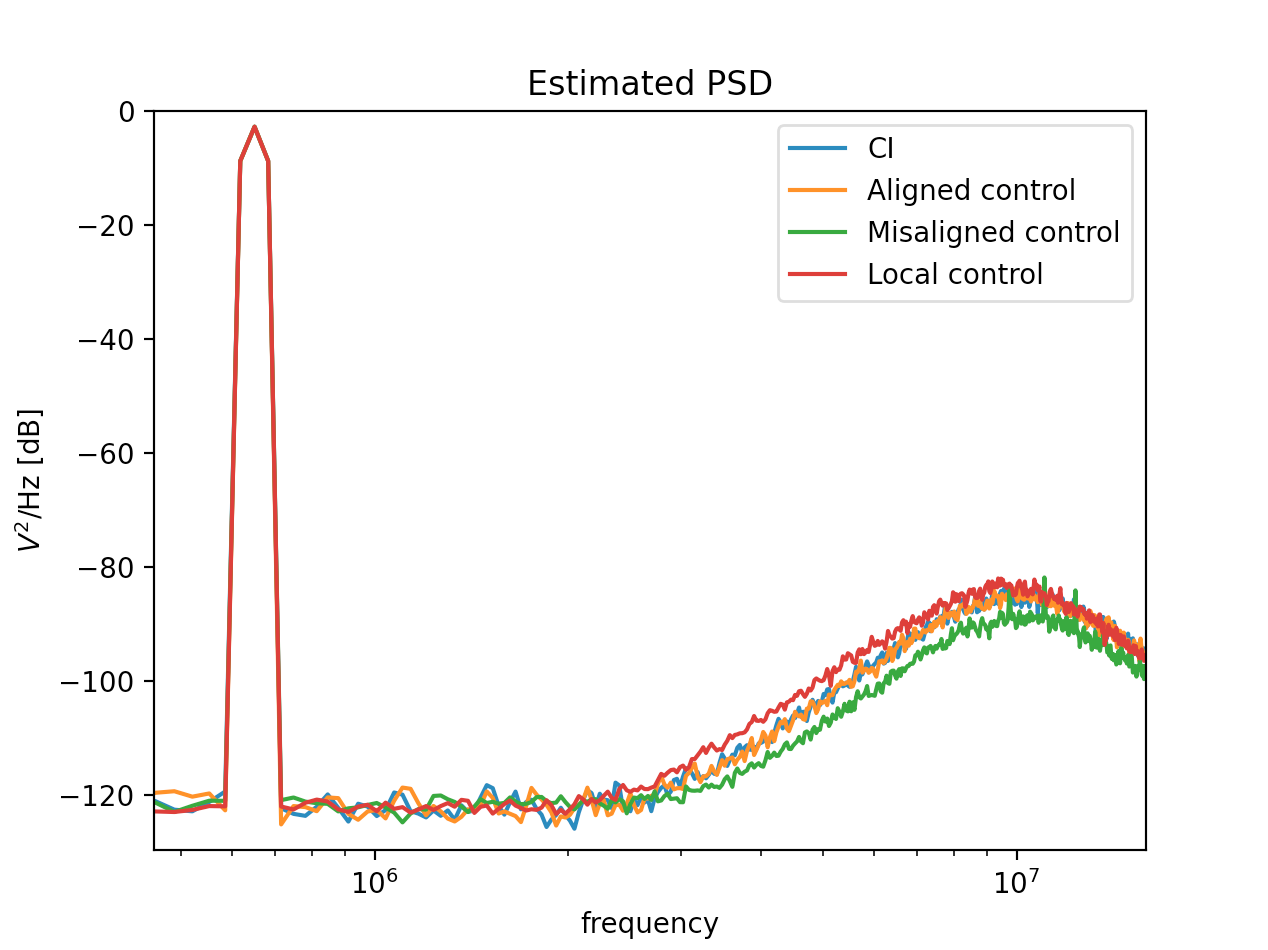
\includegraphics[width=\linewidth]{figures/05hadamard/ideal_sim.png}
    \caption{Simulation results of the proposed ADC architecture for $N=4$. The three considered choices of control matrix are compared together with the chain-of-integrators (CI) system of the same order. The input is a single sinusoidal signal with a $90\%$ full scale amplitude. }
    \label{fig:HCI_SIM1}
\end{figure}
The simulation shows that the proposed ADC performs very similar to the chain-of-integrators from chapter \ref{sec:ciadc}. Especially the aligned control configuration is almost indistinguishable from the chain-of-integrators. As the proposed Hadamard ADC is essentially a chain-of-integrators with an intermediate state rotation, completely aligning the control and signal dimensions makes this configuration essentially equal to the chain-of-integrators in the ideal case. For the two other configurations, the performance is slightly different.

As the transfer function of the all four systems are identical, the only performance difference is (in this ideal case) caused by the digital controls ability to bound the state vector. We observe from this simulation that the misaligned control seem to perform slightly better than the other configurations.

As mentioned in the introduction to this chapter, one of the main objectives of the Hadamard ADC was to distribute the mismatch sensitivity of the involved components. A mismatch simulation is performed to see how the proposed ADC performs under component mismatch, compared to the chain-of-integrator. The simulation is done by using the same parameters as in the previous, ideal simulation. Before running the system simulation, i.e. solving ($\ref{eq:hci_state_space_equations}$), all elements of the matrices $\Amat, \Bmat$ and $\Gmat$ are offset from their ideal value. The deviation is drawn randomly from a normal distribution with a standard deviation of 1\%. The reconstruction of $\utvhat$ is ultimately done using the nominal values. The presented results is obtained by averaging the output estimate of 10 simulation runs. Although this simple simulation does not completely resemble a realistic mismatch situation, it gives an indication of how the system is affected by non-ideal component values.

\begin{figure}[htbp]
    \centering
    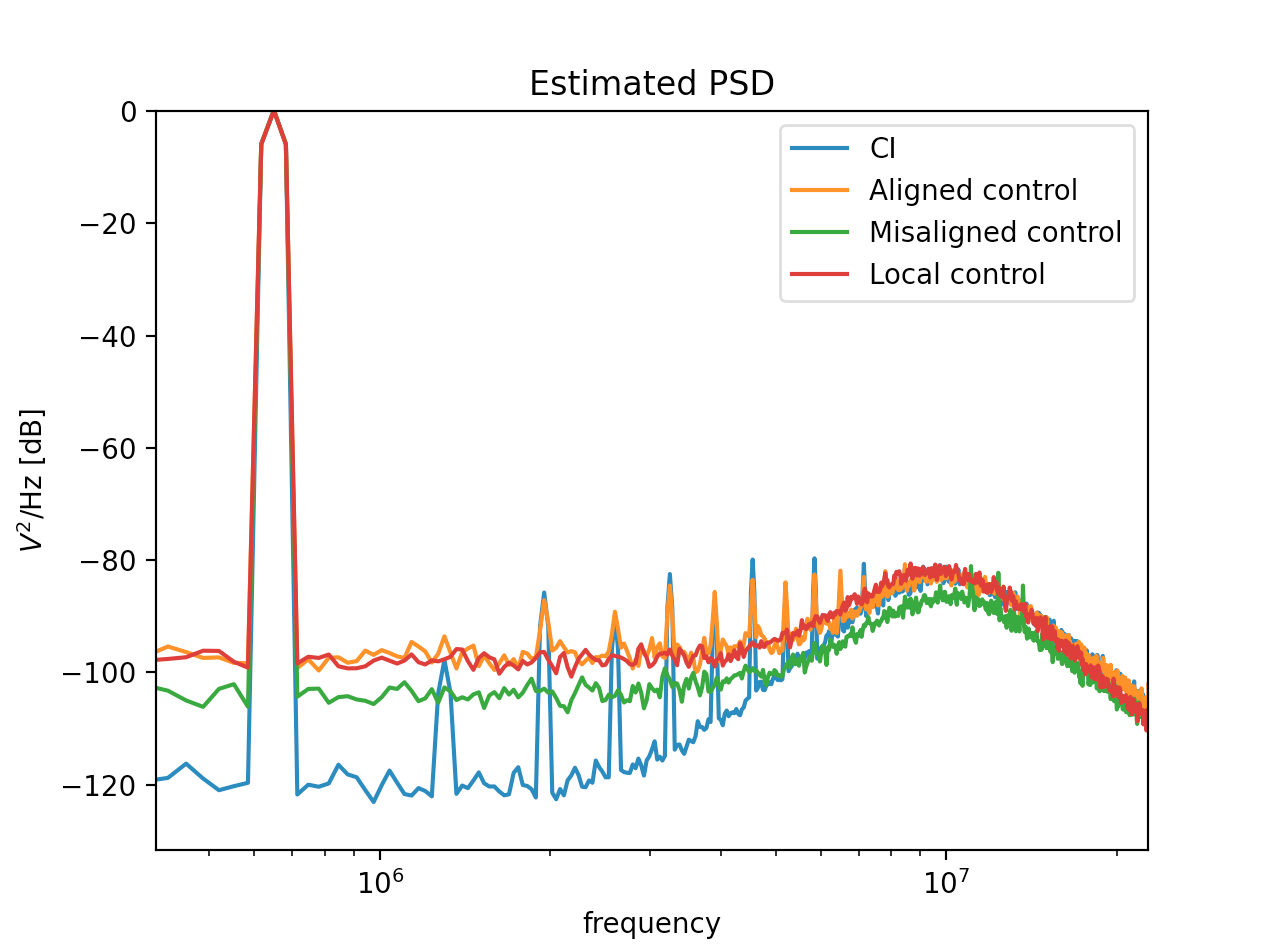
\includegraphics[width=\linewidth]{figures/05hadamard/mismatch_sim.png}
    \caption{Mismatch simulation, all parameters drawn from normal distribution with std=1\%. Comparison between different control parametrizations and the chain-of-integrator ADC}
    \label{fig:hci_mismatch_sim}
\end{figure}

The estimated PSD from this simulation is shown in figure \ref{fig:hci_mismatch_sim}. First of all, we note that the power spectrum of the chain-of-integrators suffers from significant harmonics due to the introduced mismatch. Furthermore, the different Hadamard configurations all show an increased noise floor, and the amount of harmonics differs between the control configurations. The increased noise floor might be understood from the averaging effect of the Hadamard transform. As the logical signal is offset from the physical states, the mismatch causes a leakage between the signal dimensions which appears as an increased noise floor in the spectrum.

The magnitude of this noise floor as well as the amount of harmonics differ considerably between the three control configurations. The aligned control has almost the same amount of harmonics as the chain-of-integrator. The alignment of control and signal dimensions causes mismatch in the control matrices to affect the signal dimensions separately, thereby introducing harmonics in the spectrum. On the other hand, both the local and misaligned control show essentially no harmonics in the spectrum, which might be understood from the completely or partial misalignment between control and signal dimensions. For some reason, the misaligned control produces a noise floor that is a few dB lower than that of the local control configuration.

Whether this effect of turning harmonics into an increased noise floor is favorable will depend on the application. For medical ultrasound applications, it is often the magnitude of second harmonic that is most critical, and it might favorable to accept more harmonics at the price of lower noise floor.


